\subsection{Mediator}

Nesse padrão, um objeto chamado de Mediator age como intermediário 
entre um grupo de objetos, fazendo com que qualquer interação entre 
eles seja encapsulada em um único objeto. O Mediator conhece todos 
os seus Colleagues, enquanto cada Colleague conhece apenas o 
Mediator.

Dessa forma, os objetos que precisam comunicar-se tornam-se 
mais independentes uns dos outros, simplificando a organização e 
a comunicação. A reutilização desses objetos também é mais simples 
e qualquer comportamento distribuído entre várias classes torna-se 
mais simples de ser customizável ou adaptável.

\begin{figure}[htb]
	\caption{\label{fig_grafico}Estrutura do Mediator}
	\begin{center}
	    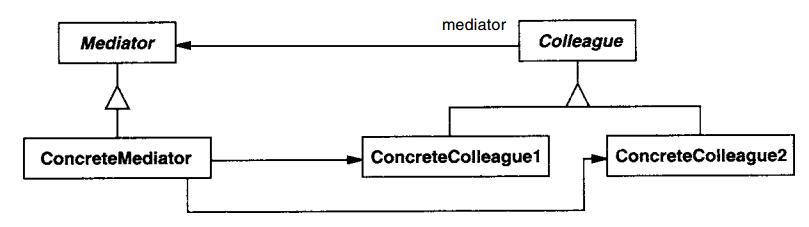
\includegraphics[scale=0.5]{5_padroes-contexto-funcional/5.3_comportamentais/5.3.05_mediator/diagram.png}
	\end{center}
\end{figure}

Exemplo Orientado a Objetos:

\begin{lstlisting}[caption={Mediator Orientação a Objetos},label=oomediator]


    
\end{lstlisting}

Contexto Funcional:

Para implementar esse padrão, é necessário tratar o objeto 
Mediator como uma função ou um conjunto de funções (uma para 
cada operação que o objeto Mediator possuiria) que recebe 
como parâmetro o valor do Colleague que realiza a operação 
e uma coleção com os outros Colleagues monitorados pelo 
Mediator.

Caso o processo de armazenar os Colleague seja trabalhoso, 
é possível encapuslar a coleção dos Colleagues em uma 
closure. Uma função deve receber a coleção e retornar 
outra função que recebe os parâmetros necessários (por 
exemplo, uma função ou valor que indique qual dos Colleagues 
é o causador da operação) e realiza de fato a operação 
nos colleagues. Enretanto, caso a lista de Colleagues 
seja alterada pela própria operação do Mediator ou por 
alguma outra modificação durante a aplicação, é necessário 
chamar a função geradora novamente para que a closure 
envolvida pela função do Mediator não fique desatualizada.

\begin{lstlisting}[caption={Mediator Funcional},label=fpmediator]
    

    
\end{lstlisting}